\documentclass[11pt,t,usepdftitle=false,aspectratio=169]{beamer}
\usepackage{biblatex}
\usepackage{color}

\addbibresource{bibliography.bib}

\usetheme[nototalframenumber,foot,logo]{uibk}

%% information for the title page
\title[Erkennung von Resampling]{Erkennung von Resampling}
\subtitle{InterpoLIE-tion - Catching lies through interpolation analysis}

\author[Dominik Barbist, Lukas Egger]{Dominik Barbist, Lukas Egger \\ \vspace{0.5em}}
\footertext{Digitale Forensik mit Bild- und Videodaten}
\date{\today}

\headerimage{3}

\begin{document}

%% this sets the first PDF bookmark and triggers generation of the title page
\section{Introduction}

\begin{frame}
	\frametitle{Übersicht}
	\begin{enumerate}
		\item \textbf{Einführung}
		\begin{itemize}
			\item Aufgabenstellung
		\end{itemize}
		\item \textbf{Beispielfall}
		\begin{itemize}
			\item Kartoffel-Contest Szenario
		\end{itemize}
		\item \textbf{Lösungsansätze}
		\begin{itemize}
			\item Exposing Digital Forgeries by Detecting Traces of Resampling
			\item Fast and Reliable Resampling Detection by Spectral Analysis
			\item Blind Authentication Using Periodic Properties of Interpolation
			\item Detection of Linear and Cubic Interpolation in JPEG Compressed Images
			\item Normalized Energy Density-Based Forensic Detection
			\item An SVD Approach to Forensic Image Resampling Detection
		\end{itemize}
	\end{enumerate}
\end{frame}

\subsection{Einführung}

\begin{frame}
	\frametitle{Einführung}
	\begin{itemize}
		\item \textbf{Aufgabenstellung:}\\
		\begin{itemize}
			\item Oft werden Bildteile während einer Manipulation skaliert, gedreht oder gestreckt. Dabei kommt Interpolation zum Einsatz, welche die Abhängigkeiten zwischen benachbarten Pixeln verändert.  
		\end{itemize} 
		\item \textbf{Motivation:} 
		\begin{itemize}
			\item Simples Bearbeitungswerkzeug, das in vielen Bildbearbeitungsprogrammen verfügbar ist
			\item Manipulationen sind oft nicht sofort erkennbar(Wenn man mit den Tools umgehen kann)
			\item Resampling Detection kann dazu beitragen, digitale Fälschungen zu identifizieren
		\end{itemize}
	\end{itemize}
\end{frame}

\subsection{Kartoffel-Contest Szenario}

\begin{frame}
	\frametitle{Kartoffel-Contest Szenario}
	\begin{columns}[T]
		\begin{column}{0.6\textwidth}
			\begin{itemize}
				\item \textbf{Online-Größenwettbewerb:} 
				\begin{itemize}
					\item Teilnehmer fotografieren größte Kartoffeln
					\item Maßband/Lineal als Größenreferenz
					\item Upload auf Contest-Plattform
				\end{itemize}
				\item \textbf{Das Problem:} 
				\begin{itemize}
					\item Skalierung der Kartoffel (größer erscheinen)
					\item Verkleinerung des Maßbands (Proportionen manipulieren)
					\item 200g-Kartoffel wird zu "500g-Riese"
				\end{itemize}
				\item \textbf{Die Herausforderung:} 
				\begin{itemize}
					\item Manipulation visuell nicht erkennbar
					\item Alle Proportionen im Bild stimmen
				\end{itemize}
			\end{itemize}
		\end{column}
		\begin{column}{0.38\textwidth}
			\centering
			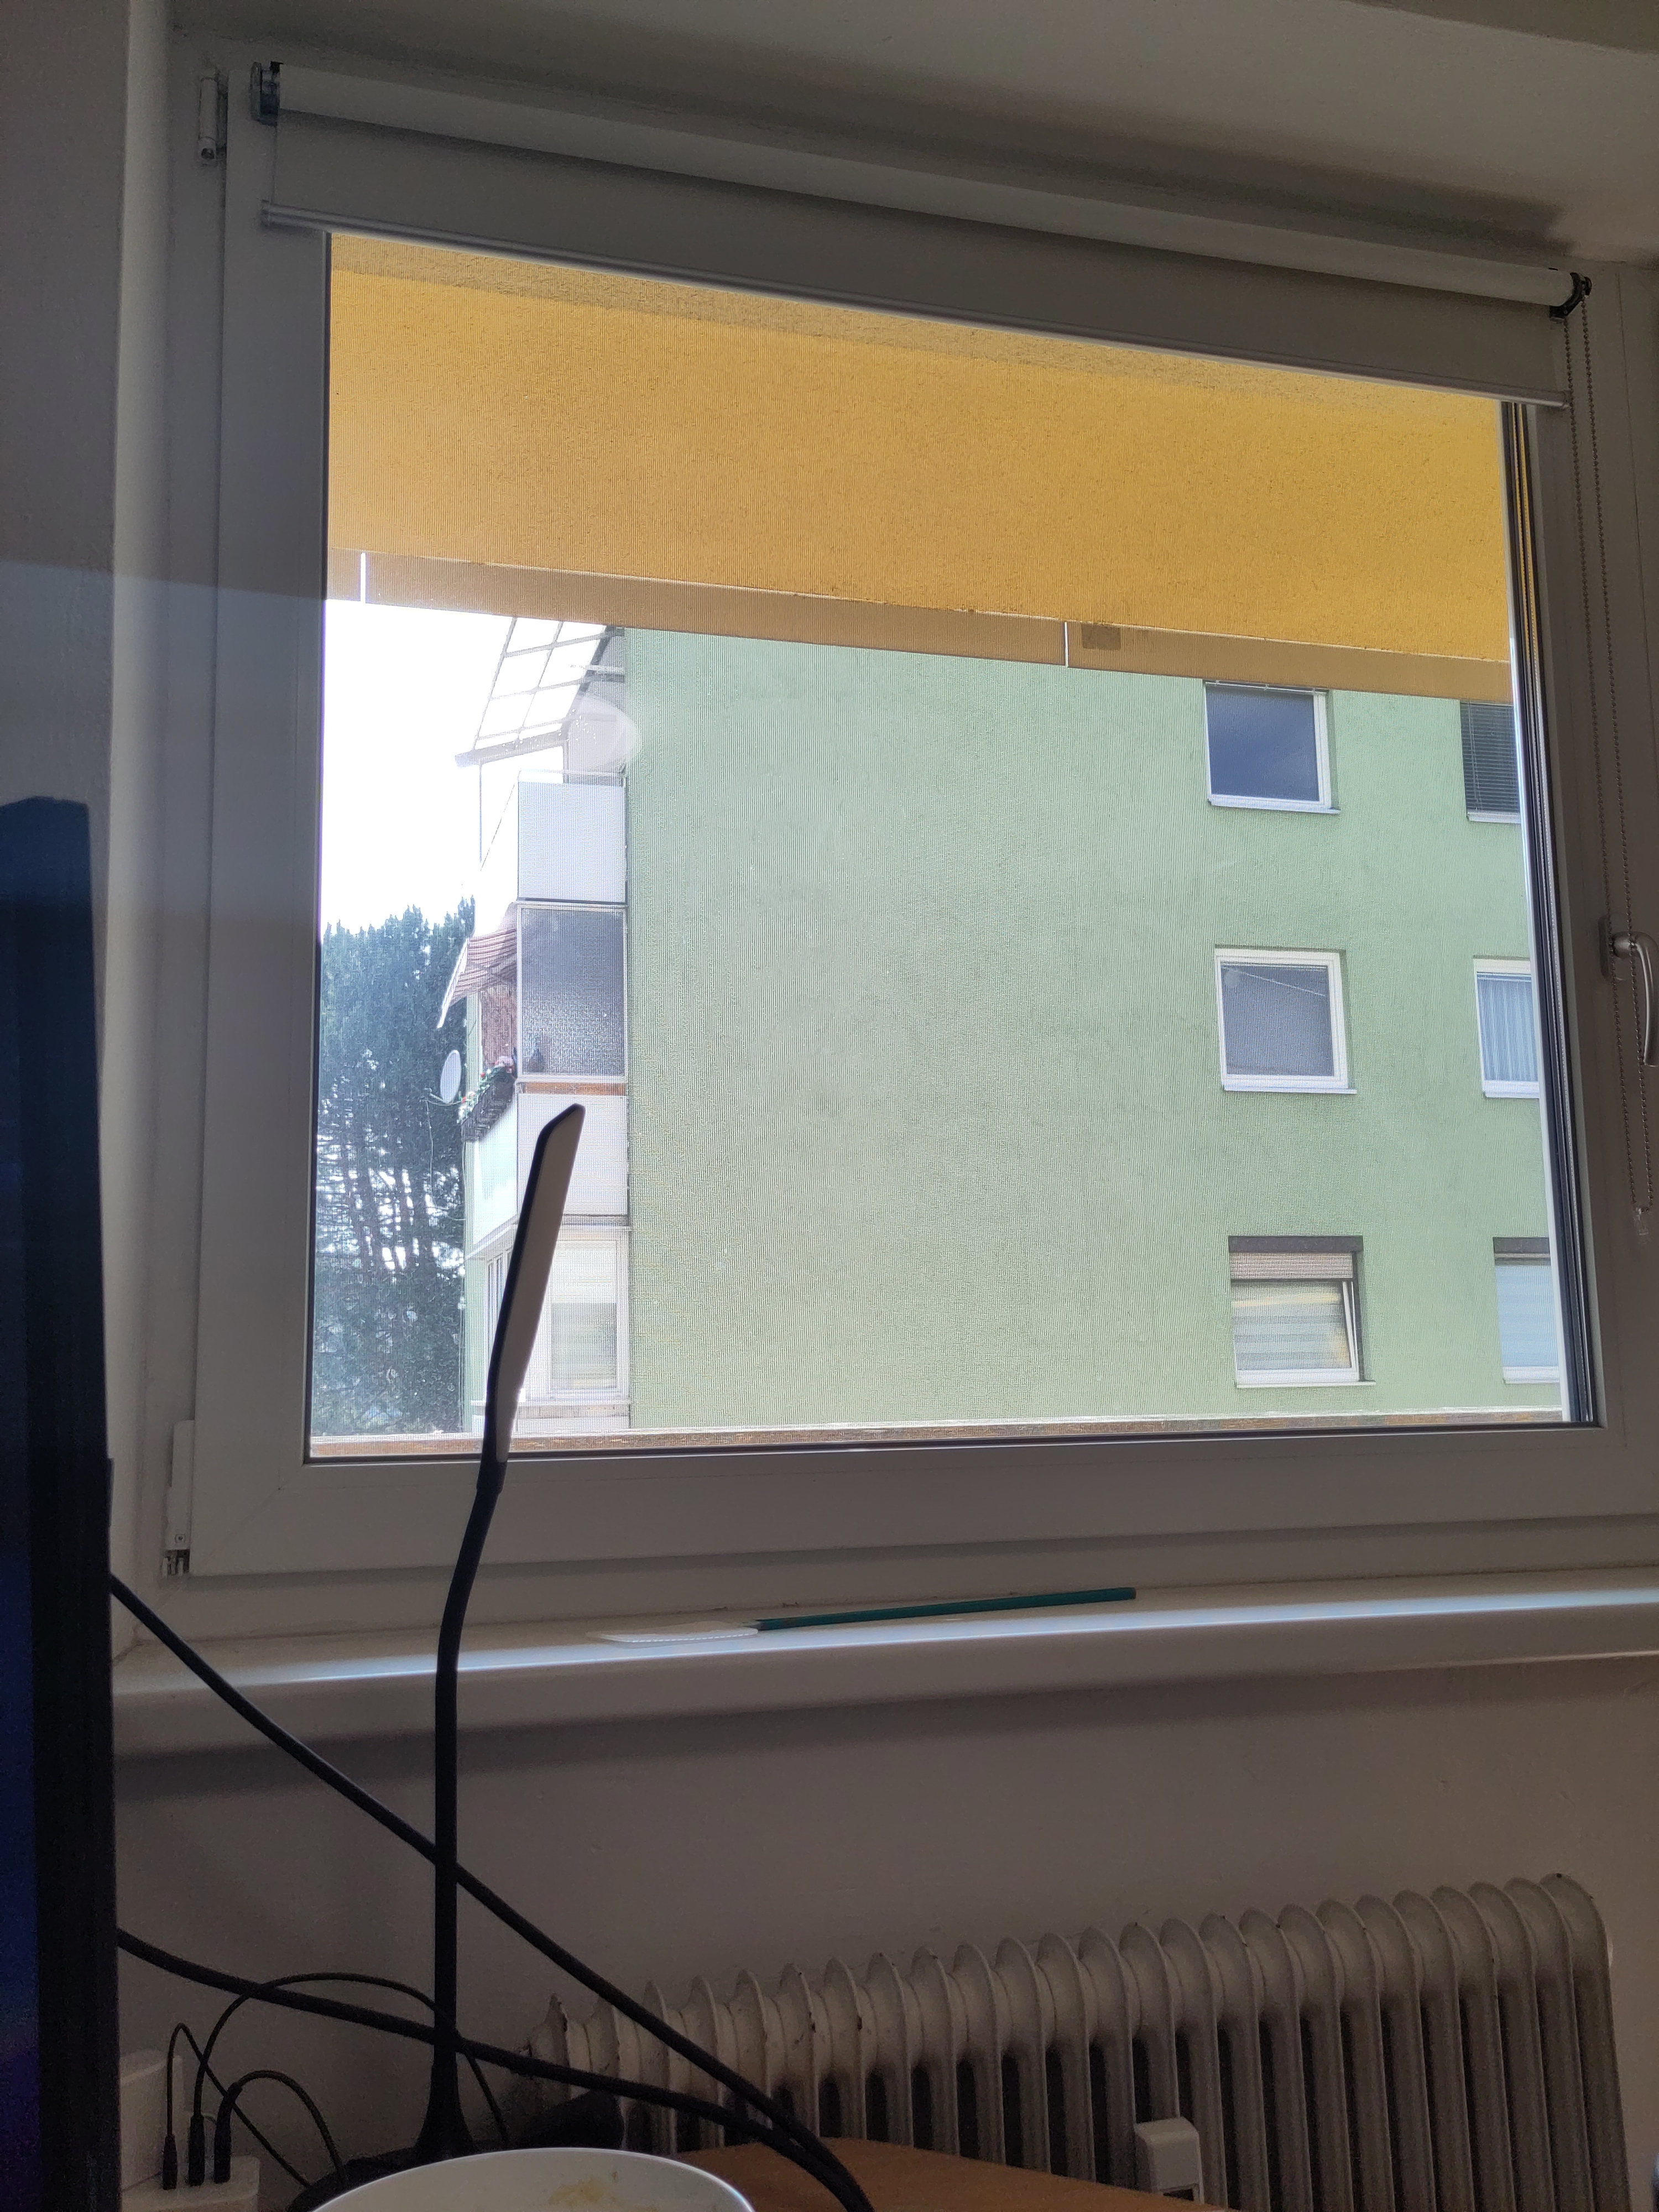
\includegraphics[width=\textwidth]{images/image_2.jpg}
			\vspace{0.5cm}
			
			\includegraphics[width=\textwidth]{images/image_2_s.jpg}
		\end{column}
	\end{columns}
\end{frame}

\subsection{Lösungsansätze}

\begin{frame}
	\frametitle{Lösungsansätze}
	\begin{itemize}
		\item \textbf{Exposing Digital Forgeries by Detecting Traces of Resampling (Popescu \& Farid, 2005):} 
		\begin{itemize}
			\item Identifikation von Resampling-Spuren mittels EM-Algorithmus
			\item Analyse der Auswirkungen auf Bilddaten
			\item \textcolor{green}{Theoretisch fundiert, vielseitig einsetzbar}
			\item \textcolor{red}{Rechenintensiv O(N²), JPEG-anfällig (Q<90)}
		\end{itemize}
		\item \textbf{Fast and Reliable Resampling Detection by Spectral Analysis (Kirchner, 2008):} 
		\begin{itemize}
			\item Nutzung der Spektralanalyse zur Erkennung von Resampling
			\item Effizienz und Zuverlässigkeit der Methode
			\item \textcolor{green}{40x schneller, vergleichbare Genauigkeit}
			\item \textcolor{red}{Weniger adaptiv, schlechter bei kleinen Blöcken}
		\end{itemize}
		\item \textbf{Blind Authentication Using Periodic Properties (Mahdian \& Saic, 2008):} 
		\begin{itemize}
			\item Authentifizierung ohne Vorwissen über das Bild
			\item Periodische Eigenschaften der Interpolation nutzen
			\item \textcolor{green}{180° Projektionsanalyse, rotationsrobust}
			\item \textcolor{red}{180 DFT-Berechnungen, viele Parameter}
		\end{itemize}
	\end{itemize}
\end{frame}

\begin{frame}
	\frametitle{Lösungsansätze (Fortsetzung)}
	\begin{itemize}
		\item \textbf{Detection of Linear and Cubic Interpolation in JPEG (Gallagher, 2005):} 
		\begin{itemize}
			\item Spezielle Fokussierung auf JPEG-Bilder
			\item Unterscheidung zwischen linearer und kubischer Interpolation
			\item \textcolor{green}{JPEG-optimiert, praktisch relevant}
			\item \textcolor{red}{Nur JPEG-Format, versagt bei Q<70}
		\end{itemize}
		\item \textbf{Normalized Energy Density-Based Forensic Detection (Feng et al., 2012):} 
		\begin{itemize}
			\item Energie-Dichte-Analyse zur Forensik mittels 19D-Feature-Vektor
			\item Normalisierung für verbesserte Genauigkeit
			\item \textcolor{green}{SVM-Klassifikation, 7500 BOSS-Bilder evaluiert}
			\item \textcolor{red}{Training erforderlich, manuelle Feature-Auswahl}
		\end{itemize}
		\item \textbf{An SVD Approach to Forensic Image Resampling Detection (Vázquez-Padín, 2015):} 
		\begin{itemize}
			\item Singular Value Decomposition (SVD) zur Resampling-Erkennung
			\item Mathematische Grundlagen und Implementierung
			\item \textcolor{green}{Effizient bei 32x32 Blöcken, mathematisch elegant}
			\item \textcolor{red}{Nur Upsampling ($\xi$ >1), parameterabhängig}
		\end{itemize}
	\end{itemize}
\end{frame}


\subsection{Zusammenfassung}

\begin{frame}
	\frametitle{Zusammenfassung}
	\begin{itemize}
		\item Resampling Detection ist ein wichtiger Aspekt der digitalen Forensik
		\item Verschiedene Ansätze bieten robuste und effiziente Lösungen
		\item Zukünftige Entwicklungen könnten die Genauigkeit und Anwendbarkeit weiter verbessern
	\end{itemize}
\end{frame}

\subsection{Quellen}
\begin{frame}
	\frametitle{Quellen}
	\printbibliography[heading=none]
\end{frame}

%% to show a last slide similar to the title slide
\title[Erkennung von Resampling]{Erkennung von Resampling}
\subtitle{InterpoLIE-tion - Catching lies through interpolation analysis}
\section{Vielen für Ihre Aufmerksamkeit!}


\end{document}